\section{Methodology}
\label{sec:method}

Given a target research idea and a set of prior ideas proposed before it, EGRD
assesses the target's novelty relative to the supplied evidence. The model
proceeds in three stages, shown in Figure~\ref{fig:framework}. Stage~A assembles the historical evidence: it selects
temporally admissible priors and summarizes how much of the target they already
account for. Stage~B decomposes the target against that evidence and represents
the uncovered contribution through two complementary components, where unit
residuals capture semantic content with insufficient historical support and
interaction residuals capture potentially novel combinations of semantic units.
Stage~C predicts an ordered novelty grade from \textsc{low} to \textsc{high}
from these residual representations.

Throughout, $[\cdot;\cdot]$ denotes concatenation, $\odot$ elementwise
multiplication, $d$ the encoder dimension, $\sigma$ the sigmoid function, and
$\varepsilon$ a small positive constant added for numerical stability. Padded
priors are masked out, and $\mathcal{V}$ denotes the non-padding positions of
the target.

\begin{figure}[t]
\centering
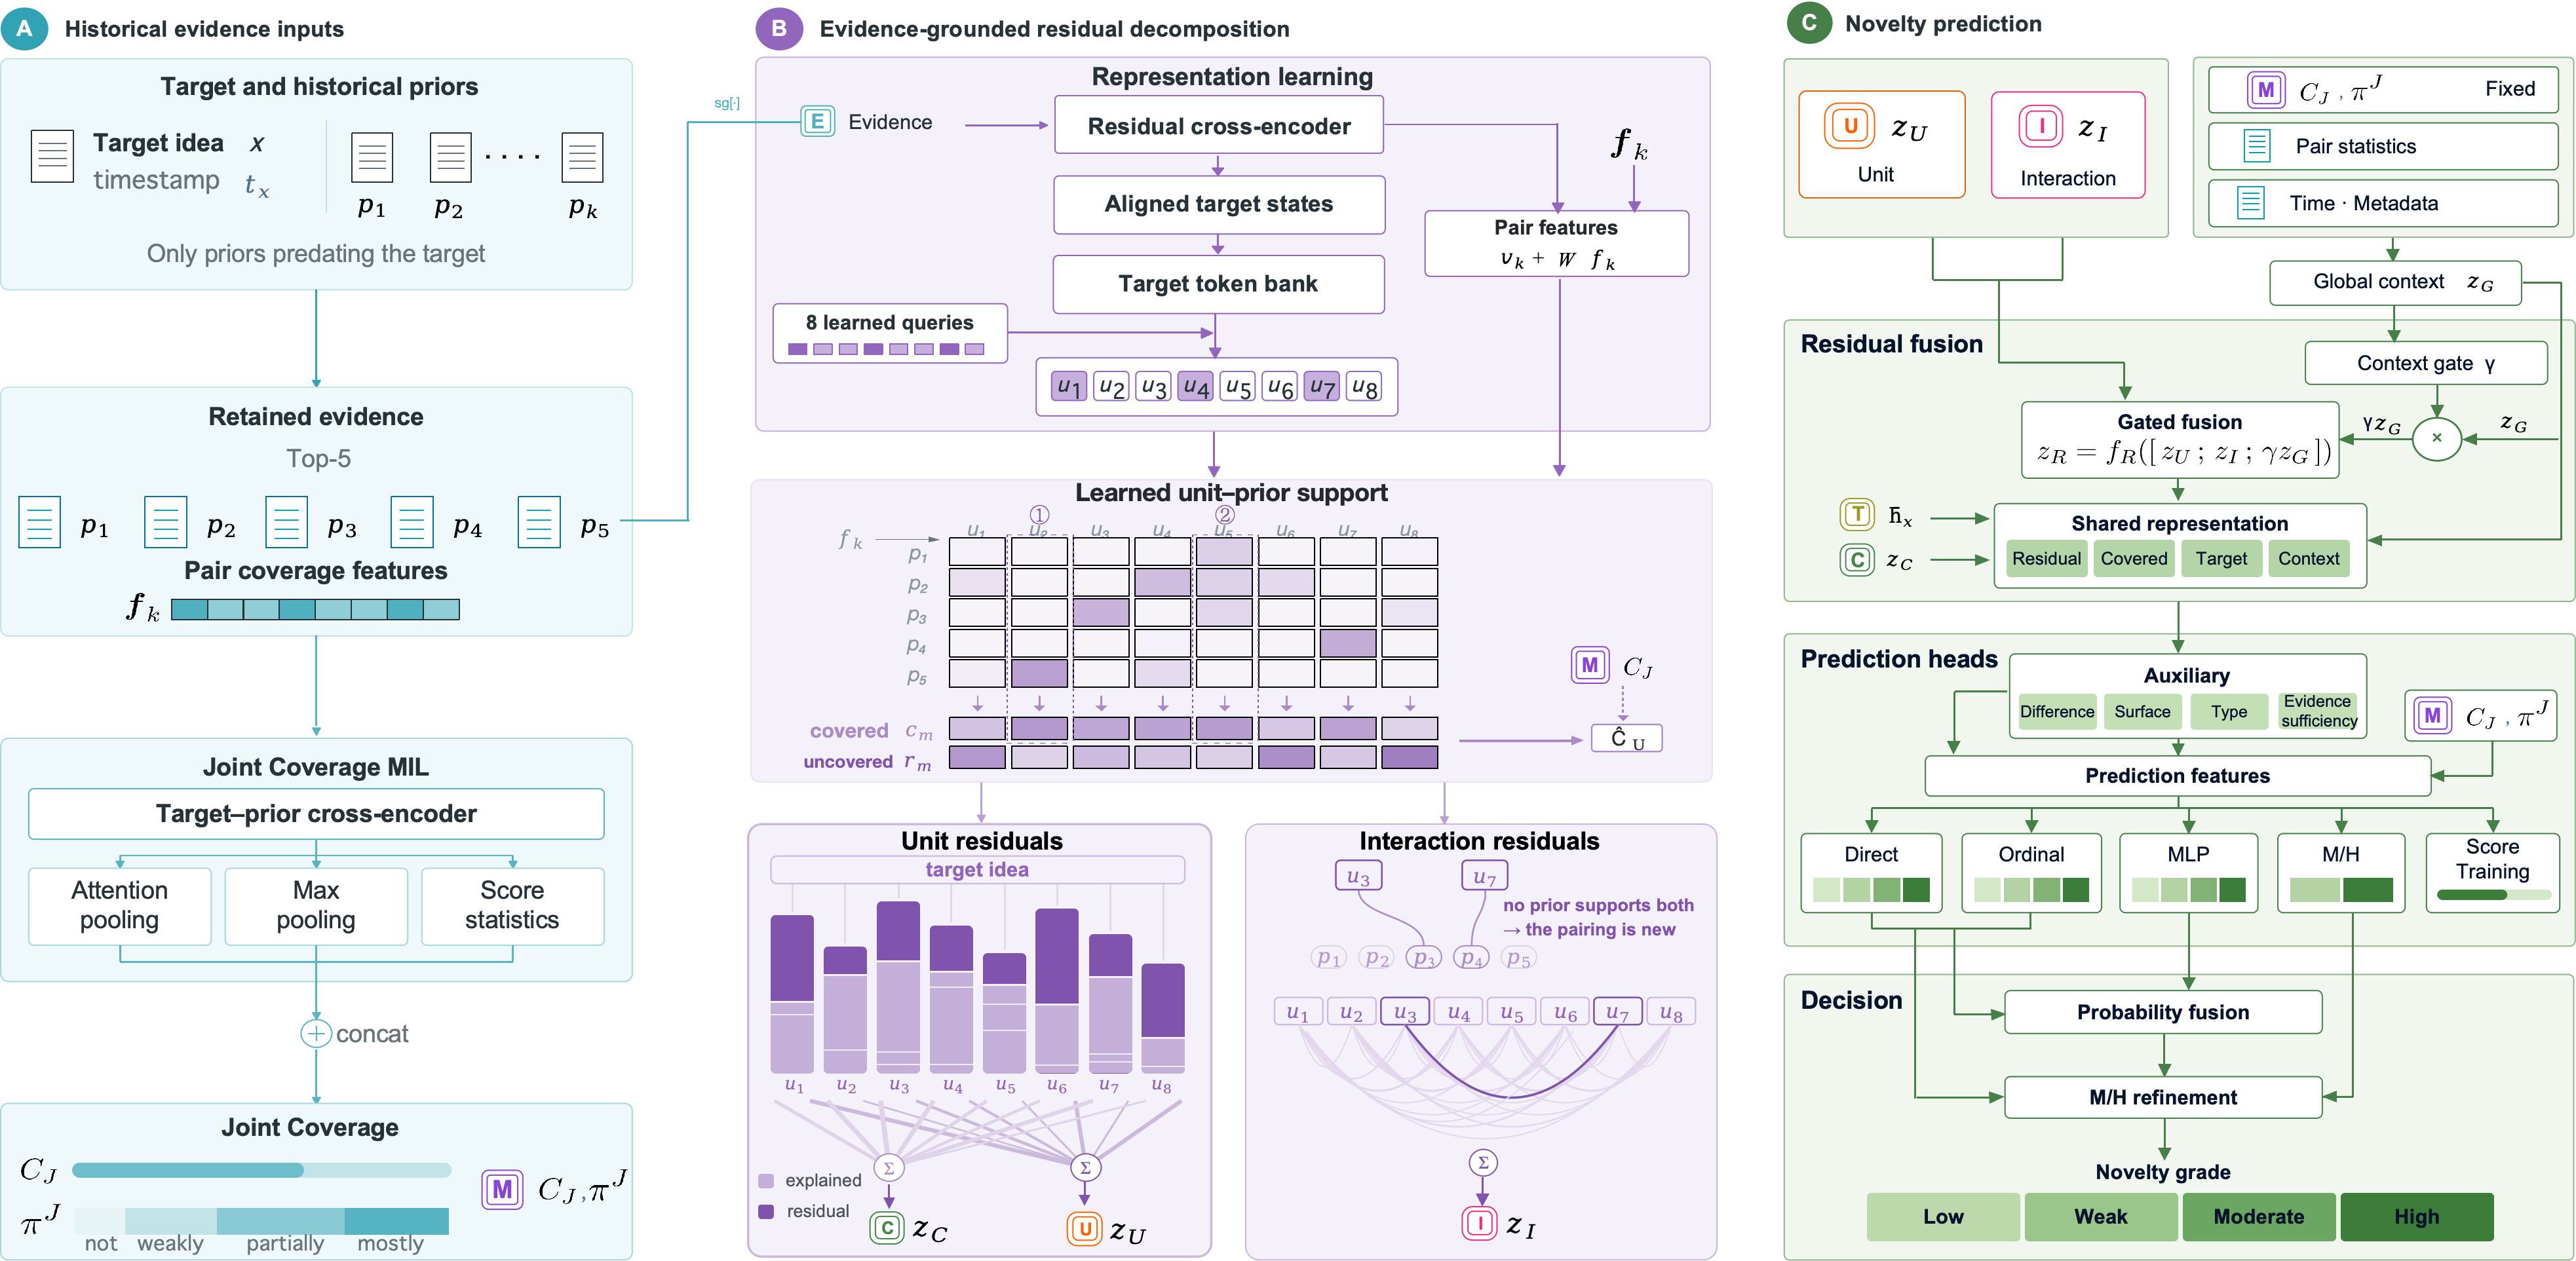
\includegraphics[width=\textwidth]{pic/framework.png}
\caption{Overview of EGRD. \textbf{(A)} Only priors predating the target are
admissible; the retained top-$K$ evidence carries pair coverage features
$\boldsymbol{f}_k$, and a multiple-instance model over target--prior pairs
predicts joint coverage $C_J$ and its four-class distribution
$\boldsymbol{\pi}^{J}$. These outputs enter the later stages as fixed inputs,
marked $\mathrm{sg}[\cdot]$. \textbf{(B)} A
residual cross-encoder builds a target token bank, which $M$ learned queries
partition into semantic units $\boldsymbol{u}_m$. A learned support matrix
$A_{km}$ aligns each unit with each prior; noisy-OR over priors gives unit
coverage $c_m$, and the complementary residual $r_m$ weights the units into
$\boldsymbol{z}_U$, with the covered part pooled into $\boldsymbol{z}_C$. The
support matrix also yields co-support $b_{ij}$, so a unit pair that no single
prior supports jointly contributes to the interaction residual
$\boldsymbol{z}_I$. \textbf{(C)} A gate modulates global context within
residual fusion; the fused representation, the covered and target
representations, and global context form a shared representation.
Auxiliary predictions and joint coverage further inform the novelty branches. Direct and ordinal probabilities enter both the fused distribution
and the moderate-to-high refinement, while the continuous score head supplies
auxiliary training supervision and is excluded from the inference-time
grading rule.}
\label{fig:framework}
\end{figure}

\subsection{Stage A: Historical Evidence Inputs}
\label{sec:method-evidence}

Stage~A assembles historical evidence and estimates how much of the target
idea that evidence collectively covers. Given a target idea $x$ with timestamp
$t_x$, we restrict candidate priors to
$\mathcal{P}_x=\{p_k\mid t_{p_k}<t_x\}$, where $t_{p_k}$ denotes the timestamp
of prior idea $p_k$. We retain the top-$K$ ranked priors, or all candidates if
fewer are available, to form the evidence set
$\mathcal{E}_x\subseteq\mathcal{P}_x$ ($K=5$ in our experiments). Each retained
prior $p_k$ is associated with coverage features $\boldsymbol{f}_k$ for the
target--prior pair.

To estimate coverage across the evidence set, we use a multiple-instance
model \citep{ilse2018attentionmil}. A cross-encoder encodes each target--prior
pair, and the model aggregates the pair representations through attention
pooling and maximum pooling. The pooled representations are concatenated
with evidence-score statistics to predict joint coverage $C_J$ and a
four-class coverage distribution $\boldsymbol{\pi}^{J}$.
Appendix~\ref{app:method-evidence} specifies the pair-scoring rule and the joint
model. The retained evidence, pair features, and coverage predictions serve
as fixed inputs to Stages~B and~C, grounding the residual decomposition and
providing coverage information for novelty prediction.

We summarize the evidence set in a global context vector $\boldsymbol{z}_G$,
a learned projection of twenty-one scalars---the scaled target timestamp,
pair-score statistics over $\mathcal{E}_x$, and the joint coverage score,
entropy, and distribution $\boldsymbol{\pi}^{J}$---concatenated with
embeddings of two target facets (aspect and contribution type).
Apart from the timestamp and the facets, $\boldsymbol{z}_G$ is a
re-encoding of the Stage~A outputs, and Stage~C consumes it as a summary of
what the evidence collectively establishes.

\subsection{Stage B: Evidence-Grounded Residual Decomposition}
\label{sec:method-decomposition}

Stage~B decomposes the target into semantic units and estimates their support
from the retained evidence. It represents the unexplained contribution through
two complementary components: unit residuals for content with limited
historical support, and interaction residuals for combinations with limited
joint support from any single prior.

\paragraph{Semantic decomposition.}
We use a residual cross-encoder initialized from the Stage~A model and trained
separately from it. For each target--prior pair, the encoder produces a pooled
representation $\boldsymbol{v}_k$, which we augment with projected pair
coverage features:
$\widetilde{\boldsymbol{v}}_k=\boldsymbol{v}_k+f_P(\boldsymbol{f}_k)$.
To obtain a shared representation of the target, we average its contextual
token states at matching positions across valid pairs, forming a token bank
$\{\boldsymbol{h}_j\}_{j=1}^{N}$, where $N$ is the number of target tokens.
We then use $M$ learned queries $\boldsymbol{q}_m$ to softly assign these tokens
to semantic units \citep{locatello2020slot} ($M=8$ in our experiments).
Queries compete for each token through a softmax over units; the resulting
assignments are then normalized over tokens within each unit:
\begin{equation}
 B_{mj}=\operatorname{softmax}_{m}
 \left(\frac{\boldsymbol{q}_m^\top\boldsymbol{h}_j}{\sqrt d}\right),
 \quad
 \alpha_{mj}=\frac{B_{mj}}{\sum_{j'\in\mathcal{V}}B_{mj'}+\varepsilon},
 \quad
 \boldsymbol{u}_m=\sum_{j\in\mathcal{V}}\alpha_{mj}\boldsymbol{h}_j.
 \label{eq:semantic-units}
\end{equation}
The units have no predefined semantic roles. A learned activity score
$v_m=\sigma(\boldsymbol{w}_v^\top\boldsymbol{u}_m+b_v)$ controls each unit's
contribution, while regularization discourages redundant token assignments.

\paragraph{Evidence-aligned unit residuals.}
\label{sec:method-unit-residual}
We estimate how strongly each prior $p_k$ supports each unit $\boldsymbol{u}_m$
through a learned support matrix:
\begin{equation}
 A_{km}=\sigma\left(f_A([
 \boldsymbol{u}_m;\widetilde{\boldsymbol{v}}_k;
 \boldsymbol{u}_m\odot\widetilde{\boldsymbol{v}}_k;
 |\boldsymbol{u}_m-\widetilde{\boldsymbol{v}}_k|;\boldsymbol{f}_k])\right),
 \label{eq:unit-support}
\end{equation}
where $f_A$ is an MLP. Support is estimated separately for every target--prior
pair, so different priors can account for different units. For
$n=|\mathcal{E}_x|$ retained priors, noisy-OR aggregates support across priors
into unit coverage $c_m$. Its complement, weighted by unit activity, defines
the residual weight $r_m$:
\begin{equation}
 c_m=1-\prod_{k=1}^{n}(1-A_{km}),\qquad
 r_m=v_m(1-c_m),\qquad
 \boldsymbol{z}_U=\frac{1}{M}\sum_m r_m\boldsymbol{u}_m.
 \label{eq:unit-residual}
\end{equation}
Noisy-OR lets several partially relevant priors jointly cover a unit that none
of them covers alone. We use it as a differentiable aggregation rule, not as a
claim that the priors are independent sources of support
(Appendix~\ref{app:method-representations}).
An active unit with little historical support receives a large residual
weight in $\boldsymbol{z}_U$. We normalize by the fixed number of units $M$
rather than by $\sum_mr_m$, so that the pooled representation retains the total
residual mass instead of dividing it away. We also pool
the supported content as
$\boldsymbol{z}_C=M^{-1}\sum_m v_mc_m\boldsymbol{u}_m$.
To connect unit coverage to supervision, a learned, activity-weighted pooling
of $c_m$ reconstructs joint coverage $\widehat C_U$, supervised by annotated
coverage and the fixed Stage~A prediction. The entries of the support matrix
are latent strengths learned without unit-level alignment labels.

\paragraph{Interaction residuals.}
\label{sec:method-interaction}
Units that are individually covered may still form a new combination. For
each unit pair $i<j$, an MLP maps their concatenation, elementwise product,
and absolute difference to an interaction representation
$\boldsymbol{t}_{ij}$, and a sigmoid head predicts its strength $g_{ij}$.
We measure historical co-support by the largest product of the two units'
support strengths within a single prior. The co-support score $b_{ij}$,
interaction residual weight $r_{ij}$, and pooled representation are
\begin{equation}
 b_{ij}=\max_k A_{ki}A_{kj},\qquad
 r_{ij}=g_{ij}(1-b_{ij}),\qquad
 \boldsymbol{z}_I=\sum_{i<j}\eta_{ij}r_{ij}\boldsymbol{t}_{ij},
 \label{eq:interaction-residual}
\end{equation}
where the learned attention $\eta_{ij}$ includes a
$\log(r_{ij}+\varepsilon)$ bias that favors pairs with larger residual
weights. When different priors support the two units but no single prior
strongly supports both, their unit residuals can be small while their
interaction residual remains large, provided that $g_{ij}$ is high.
An auxiliary classifier on $\boldsymbol{z}_I$ is trained with idea-level
labels for nontrivial combinations. Co-support serves as a proxy for an
existing combination: a prior that supports both units need not cover the
specific way they are combined in the target.
Appendix~\ref{app:method-representations} provides the detailed pooling
equations.

\subsection{Stage C: Novelty Prediction}
\label{sec:method-prediction}

Stage~C predicts an ordered novelty grade from the residual representations
and the evidence context. To account for evidence availability and uncertainty,
we condition residual fusion on the global context $\boldsymbol{z}_G$ defined
in Section~\ref{sec:method-evidence}. A learned gate $\gamma$ takes
$\boldsymbol{z}_U$, $\boldsymbol{z}_I$, $\boldsymbol{z}_G$, and the entropy of
the Stage~A coverage prediction as inputs and scales the context within the
residual branch:
\begin{equation}
 \boldsymbol{z}_R=f_R([\boldsymbol{z}_U;\boldsymbol{z}_I;
                       \gamma\boldsymbol{z}_G]),\qquad
 \boldsymbol{h}=\operatorname{LayerNorm}([
 \boldsymbol{z}_R;\boldsymbol{z}_C;\bar{\boldsymbol{h}}_x;\boldsymbol{z}_G]),
 \label{eq:residual-fusion}
\end{equation}
where $\bar{\boldsymbol{h}}_x$ is obtained by masked mean pooling over the target token bank.
The shared representation $\boldsymbol{h}$ retains the covered content,
the target representation, and a direct path for global context. The gate
therefore controls context only within residual fusion.

Auxiliary heads predict substantive difference, surface change, evidence
sufficiency, and residual type. These predictions, together with
$\boldsymbol{h}$ and joint coverage, form the inputs to three novelty
branches: a direct linear classifier, a cumulative ordinal head that models
grade order, and a two-layer MLP classifier. Each branch produces a
four-class distribution, and their convex mixture determines an initial
grade. A moderate-to-high refinement upgrades an initial \textsc{moderate}
prediction when a weighted combination of the direct and ordinal
\textsc{high}-class probabilities and a separate binary-head score exceeds
a threshold. The mixture weights and refinement threshold are selected on
development data and fixed for testing
(Appendix~\ref{app:method-heads}). A separate continuous novelty head provides
auxiliary supervision during training; its output is not used in the
inference-time grading rule.

\subsection{Training Objective}
\label{sec:method-learning}

We initialize the residual encoder from the Stage~A joint-coverage checkpoint
and jointly optimize it with the decomposition and prediction modules in
Stages~B and~C, while keeping the Stage~A models fixed. The objective combines
classification of the novelty grade and the residual type, supervision of a
family of annotated scalar quantities, and regularization of the
decomposition.

Let $\mathcal{A}=\{\Delta,S,E,C,\nu\}$ index the annotated scalars---the
substantive difference, surface change, and evidence sufficiency read off the
auxiliary heads, the reconstructed coverage $\widehat C_U$, and the continuous
novelty score. Each contributes a smooth-$L_1$ level loss $\mathcal{L}_a$
against its annotation. Level losses alone leave these heads free to settle on
the median of their target, so we also supervise their order: the ranking terms
of $\Delta$, $S$, $E$, and $C$ are collected into a single
$\mathcal{L}_{\mathrm{rank}}$, while the novelty score carries its own ranking
term inside $\mathcal{L}_{\nu}$. The objective is
\begin{equation}
 \mathcal{L}=\sum_{a\in\mathcal{A}}\lambda_{a}\mathcal{L}_{a}
 +\lambda_{\mathrm{rank}}\mathcal{L}_{\mathrm{rank}}
 +\lambda_{\mathrm{nov}}\mathcal{L}_{\mathrm{nov}}
 +\lambda_{\mathrm{type}}\mathcal{L}_{\mathrm{type}}
 +\lambda_{\mathrm{dec}}\mathcal{L}_{\mathrm{dec}}
 +\lambda_{\mathrm{var}}\mathcal{L}_{\mathrm{var}}.
 \label{eq:training-objective}
\end{equation}
Here $\mathcal{L}_{\mathrm{nov}}$ supervises the three novelty branches, their
fused distribution, and the moderate-to-high head, and
$\mathcal{L}_{\mathrm{type}}$ supervises residual categories and nontrivial
combinations. Beyond its level loss, the coverage term $\mathcal{L}_{C}$ adds a
consistency loss against the fixed Stage~A prediction, assigning less
consistency weight to predictions with higher entropy.
$\mathcal{L}_{\mathrm{dec}}$ regularizes the decomposition against redundant
token assignments and unused units, and $\mathcal{L}_{\mathrm{var}}$ is a
variance floor that keeps the unit coverages from coinciding.
Appendix~\ref{app:method-training} defines each term and reports the
coefficients $\lambda$.
